\documentclass[aspectratio=169]{../latex_main/tntbeamer}  % you can pass all options of the beamer class, e.g., 'handout' or 'aspectratio=43'
\usepackage{dsfont}
\usepackage{bm}
\usepackage[english]{babel}
\usepackage[T1]{fontenc}
%\usepackage[utf8]{inputenc}
\usepackage{graphicx}
\graphicspath{ {./figures/} }
\usepackage{algorithm}
\usepackage[ruled,vlined,algo2e,linesnumbered]{algorithm2e}
\usepackage{hyperref}
\usepackage{booktabs}
\usepackage{mathtools}

\usepackage{amsmath,amssymb}

\DeclareMathOperator*{\argmax}{arg\,max}
\DeclareMathOperator*{\argmin}{arg\,min}

\usepackage{amsbsy}
\newcommand{\vect}[1]{\bm{#1}}
%\newcommand{\vect}[1]{\boldsymbol{#1}}

\usepackage{pgfplots}
\pgfplotsset{compat=1.16}
\usepackage{tikz}
\usetikzlibrary{trees} 
\usetikzlibrary{shapes.geometric}
\usetikzlibrary{positioning,shapes,shadows,arrows,calc,mindmap}
\usetikzlibrary{positioning,fadings,through}
\usetikzlibrary{decorations.pathreplacing}
\usetikzlibrary{intersections}
\pgfdeclarelayer{background}
\pgfdeclarelayer{foreground}
\pgfsetlayers{background,main,foreground}
\tikzstyle{activity}=[rectangle, draw=black, rounded corners, text centered, text width=8em]
\tikzstyle{data}=[rectangle, draw=black, text centered, text width=8em]
\tikzstyle{myarrow}=[->, thick, draw=black]

% Define the layers to draw the diagram
\pgfdeclarelayer{background}
\pgfdeclarelayer{foreground}
\pgfsetlayers{background,main,foreground}

% Requires XeLaTeX or LuaLaTeX
%\usepackage{unicode-math}

\usepackage{fontspec}
%\setsansfont{Arial}
\setsansfont{RotisSansSerifStd}[ 
Path=../latex_main/fonts/,
Extension = .otf,
UprightFont = *-Regular,  % or *-Light
BoldFont = *-ExtraBold,  % or *-Bold
ItalicFont = *-Italic
]
\setmonofont{Cascadia Mono}[
Scale=0.8
]

% scale factor adapted; mathrm font added (Benjamin Spitschan @TNT, 2021-06-01)
%\setmathfont[Scale=1.05]{Libertinus Math}
%\setmathrm[Scale=1.05]{Libertinus Math}

% other available math fonts are (not exhaustive)
% Latin Modern Math
% XITS Math
% Libertinus Math
% Asana Math
% Fira Math
% TeX Gyre Pagella Math
% TeX Gyre Bonum Math
% TeX Gyre Schola Math
% TeX Gyre Termes Math

% Literature References
\newcommand{\lit}[2]{\href{#2}{\footnotesize\color{black!60}[#1]}}

%%% Beamer Customization
%----------------------------------------------------------------------
% (Don't) Show sections in frame header. Options: 'sections', 'sections light', empty
\setbeamertemplate{headline}{empty}

% Add header logo for normal frames
\setheaderimage{
	% 
\includegraphics[height=\logoheight]{figures/TNT_darkv4.pdf}
	
\includegraphics[height=\logoheight]{../latex_main/figures/luh_logo_rgb_0_80_155.pdf}
	% 
\includegraphics[height=\logoheight]{figures/logo_tntluh.pdf}
}

% Header logo for title page
\settitleheaderimage{
	% 
\includegraphics[height=\logoheight]{figures/TNT_darkv4.pdf}
	
\includegraphics[height=\logoheight]{../latex_main/figures/luh_logo_rgb_0_80_155.pdf}
	% 
\includegraphics[height=\logoheight]{figures/logo_tntluh.pdf}
}

% Title page: tntdefault 
\setbeamertemplate{title page}[tntdefault]  % or luhstyle
% Add optional title image here
%\addtitlepageimagedefault{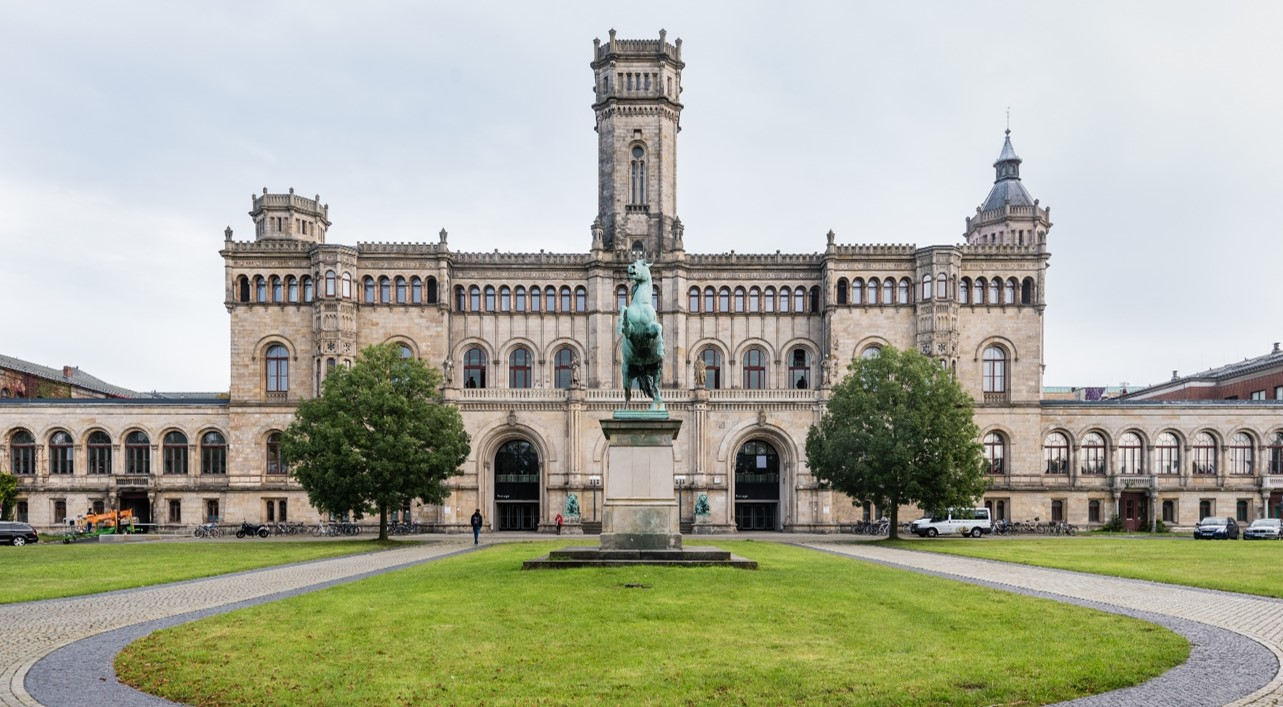
\includegraphics[width=0.65\textwidth]{figures/luh_default_presentation_title_image.jpg}}

% Title page: luhstyle
% \setbeamertemplate{title page}[luhstyle]
% % Add optional title image here
% \addtitlepageimage{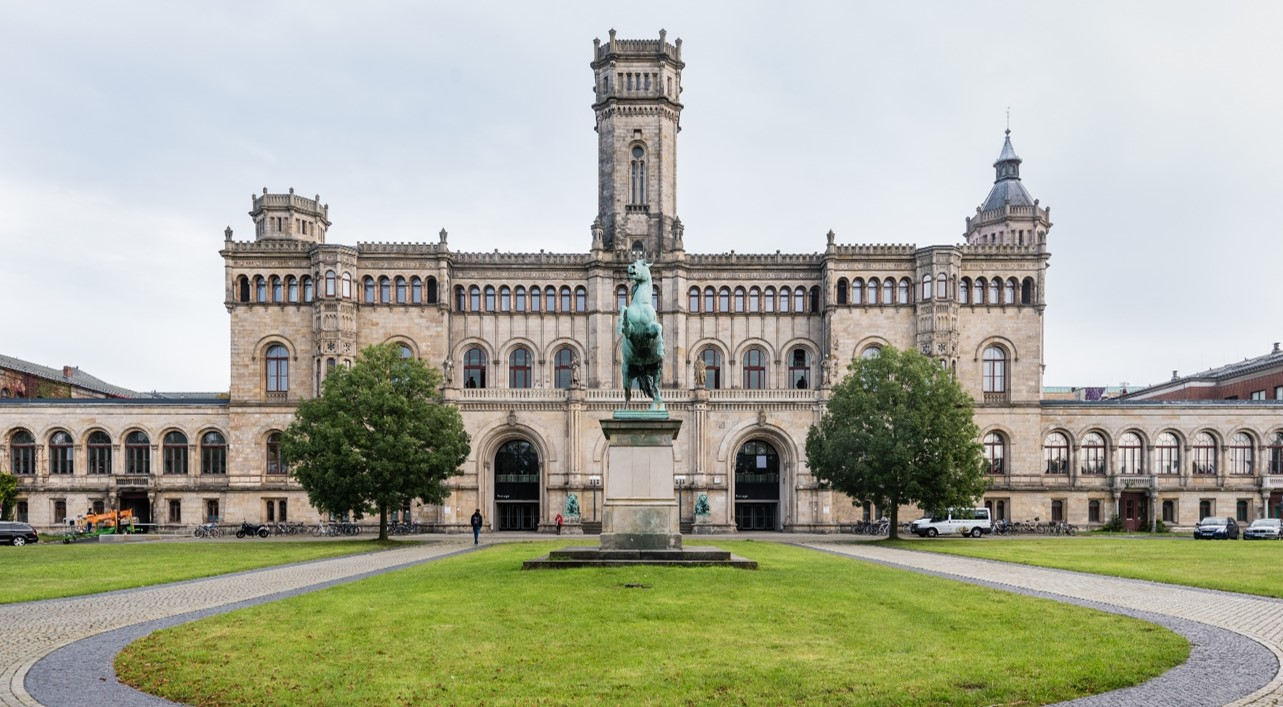
\includegraphics[width=0.75\textwidth]{figures/luh_default_presentation_title_image.jpg}}

\author[Abedjan \& Lindauer]{Ziawasch Abedjan \& Marius Lindauer\\[1em]
	
\includegraphics[height=\logoheight]{../latex_main/figures/luh_logo_rgb_0_80_155.pdf}\qquad
	
\includegraphics[height=\logoheight]{../latex_main/figures/DBIS_Kurzlogo.png}\qquad

\includegraphics[height=\logoheight]{../latex_main/figures/TNT_darkv4}\qquad

\includegraphics[height=\logoheight]{../latex_main/figures/L3S.jpg}	}
\date{Summer Term 2022; \hspace{0.5em} {
\includegraphics[height=1.5em]{../latex_main/figures/Cc-by-nc-sa_icon.svg.png}}; based on \href{https://ds100.org/fa21/}{[DS100]}
}


%%% Custom Packages
%----------------------------------------------------------------------
% Create dummy content
\usepackage{blindtext}

% Adds a frame with the current page layout. Just call \layout inside of a frame.
\usepackage{layout}


%%% Macros
%\renewcommand{\vec}[1]{\mathbf{#1}}
% \usepackage{bm}
%\let\vecb\bm

\title[Introduction]{DS: Logistic Regression, Classification}
\subtitle{Linear separability, regularization}

\graphicspath{ {./figure/} }
%\institute{}


\begin{document}
	
	\maketitle
	\begin{frame}{Question}
	    \begin{columns}
	        \begin{column}{.5\textwidth}
	              Suppose we’re training a single-parameter logistic regression model on the data to the right.\\
	              \bigskip
	              What $\theta$ minimizes mean cross-entropy loss? \\
	              \bigskip
	              $\hat{\theta} = -1$\\
	              $\hat{\theta} = 1$\\
	              $\hat{\theta} \rightarrow -\infty$\\
	              $\hat{\theta} \rightarrow \infty$\\
	        \end{column}
	        
	        
	        
	        \begin{column}{.5\textwidth}
	                \begin{figure}
	                    \centering
	                    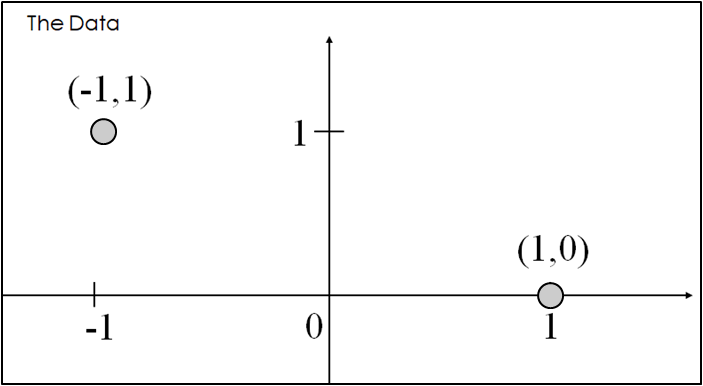
\includegraphics[scale=.5]{Bild40}
	                \end{figure}
	        \end{column}
	    \end{columns}
	    
	\end{frame}
	
	
	\begin{frame}{Question}
	    \begin{columns}
	        \begin{column}{.5\textwidth}
	              Suppose we’re training a single-parameter logistic regression model on the data to the right.\\
	              \bigskip
	              What $\theta$ minimizes mean cross-entropy loss?\\
	              \bigskip
	              $\hat{\theta} \rightarrow -\infty$
	        \end{column}
	        
	        
	        
	        \begin{column}{.5\textwidth}
	                \begin{figure}
	                    \centering
	                    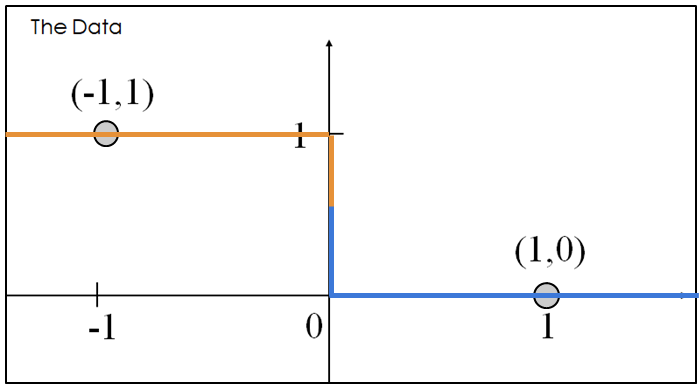
\includegraphics[scale=.35]{Bild41}
	                \end{figure}
	                
	        \end{column}
	    \end{columns}
	    \bigskip
	    $\hat{y} = f_\theta (x) = P(Y=1|x) = \sigma (x\theta) \hspace{1cm} \sigma (t) = \frac{1}{1 + e^{-t}}$
	\end{frame}
	
	
	\begin{frame}{Loss surface}
    

	    \begin{columns}
	        \begin{column}{.5\textwidth}
	            On the right is the loss surface for mean cross-entropy loss.
	            \begin{itemize}
	                \item Gradient descent will (correctly) push our guess for theta towards negative infinity.
	                \item It’s almost impossible to see, but that’s not a plateau – loss keeps decreasing and decreasing to the left.
	                \begin{itemize}
	                    \item Loss approaches 0.
	                \end{itemize}
	                \item Why is an infinitely large theta a bad idea? (     $\hat{\theta} \rightarrow -\infty$             )

	            \end{itemize}  
	        \end{column}
	        
	        
	        
	        \begin{column}{.5\textwidth}
	                \begin{figure}
	                    \centering
	                    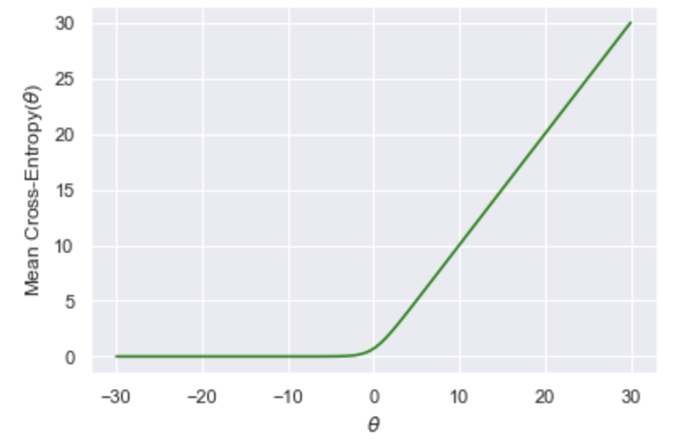
\includegraphics[scale=.5]{Bild42}
	                \end{figure}
	                
	        \end{column}
	    \end{columns}
	 \end{frame}
	 
	 
	 \begin{frame}{Issues with large parameters}
	             Why is an infinitely large theta a bad idea? (     $\hat{\theta} \rightarrow -\infty$             )
	            \begin{itemize}
	                \item A single wrong prediction will have infinite loss.
	                \item “Overconfident”.
	            \end{itemize}  
	                \begin{figure}
	                    \centering
	                    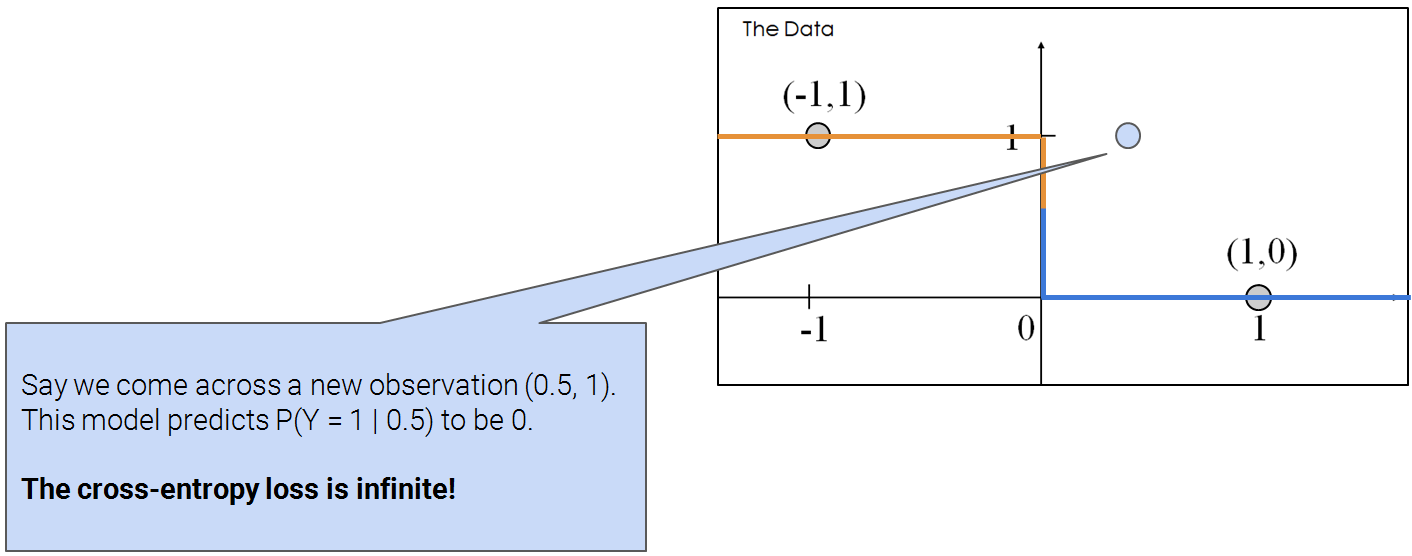
\includegraphics[scale=.33]{Bild43}
	                \end{figure}
	 \end{frame}
	 
	 
	 
	 \begin{frame}{Linear separability}
	    \begin{columns}
	        \begin{column}{.5\textwidth}
	            Points are linearly separable if we can correctly separate the classes with a line.\\
	            When considering linear separability, we ignore the class label. 
	            \begin{itemize}
	                \item The data to the left has only one feature, so it is 1D.
	                \item We are looking for a degree 0 “hyperplane” to separate them, which is a vertical line.
	            \end{itemize}  
	        \end{column}
	        
	        
	        
	        \begin{column}{.5\textwidth}
	                \begin{figure}
	                    \centering
	                    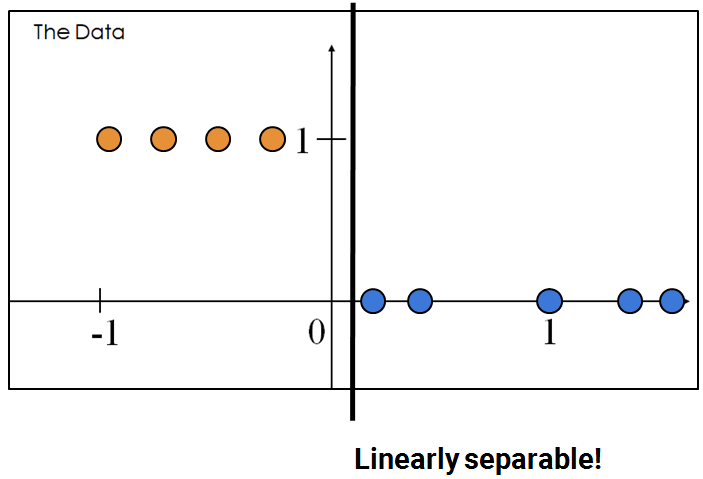
\includegraphics[scale=.35]{Bild44}
	                \end{figure}
	                
	        \end{column}
	    \end{columns}
	 \end{frame}
	 
	  \begin{frame}{Linear separability}
	    \begin{columns}
	        \begin{column}{.5\textwidth}
	            Points are linearly separable if we can correctly separate the classes with a line.\\
	            When considering linear separability, we ignore the class label. 

	            \begin{itemize}
	                \item The data to the left has only one feature, so it is 1D.
	                \item We are looking for a degree 0 “hyperplane” to separate them, which is a vertical line.
	            \end{itemize}  
	        \end{column}
	        
	        
	        
	        \begin{column}{.5\textwidth}
	                \begin{figure}
	                    \centering
	                    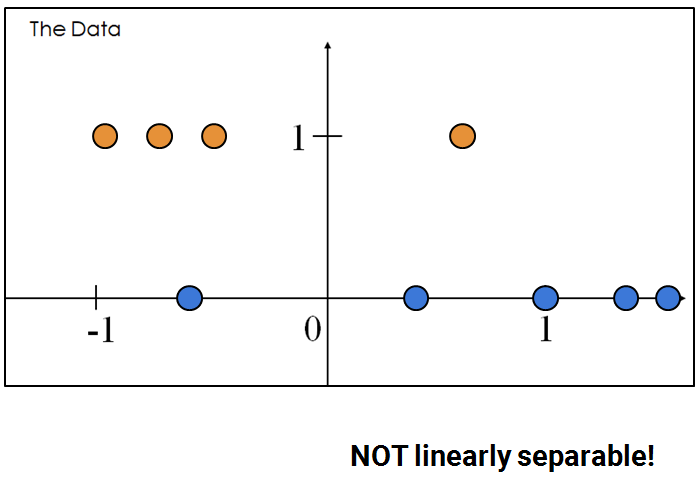
\includegraphics[scale=.35]{Bild45}
	                \end{figure}
	                
	        \end{column}
	    \end{columns}
	 \end{frame}
	 
	 
	  \begin{frame}{Linear separability in 2D}
	             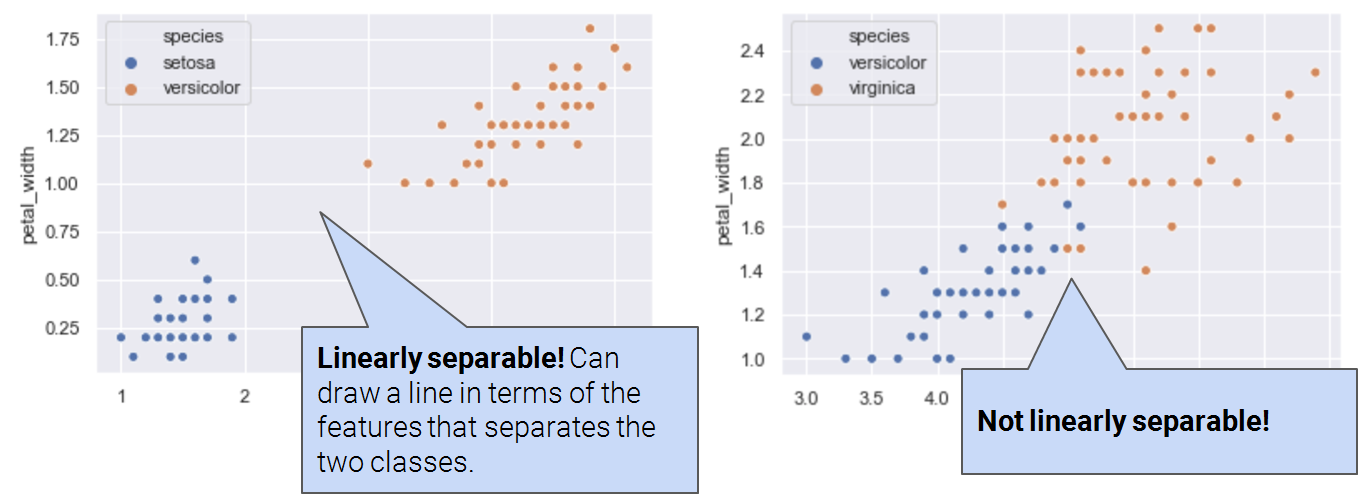
\includegraphics[scale=.4]{Bild46}\\
	             More formally: A set of d-dimensional points is linearly separable if we can draw a degree d-1 hyperplane (line) that separates the points perfectly.

	 \end{frame}
	 
	 
	 \begin{frame}{Regularized logistic regression}
	     \begin{itemize}
	         \item If our training data is linearly separable, some of our weights will diverge to infinity (either positive or negative).
	         \begin{itemize}
	             \item This is because our numeric solver (e.g. gradient descent) will keep “rolling” further and further down the loss surface.
	             \item Will eventually stop at some excessively large weight.
	         \end{itemize}
	         \item To avoid large weights, we use regularization.
	         \begin{itemize}
	             \item As with linear regression, we should standardize our features before applying regularization.
	         \end{itemize}
	         \item For instance, using L2 regularization, our objective function becomes:
	     \end{itemize}
	     \begin{equation*}
	         R(\theta) = -\frac{1}{n}\sum\limits_{i=1}^n(y_i\log(\sigma (\mathbb{X}_i^T\theta)) + (1 - y_i)\log(1-\sigma (\mathbb{X}_i^T\theta))) + \lambda\sum\limits_{i=1}^p\theta^2_i
	     \end{equation*}
	 \end{frame}
	 
	 
	 \begin{frame}{Regularized logistic regression}
	    \begin{figure}
	        \centering
	        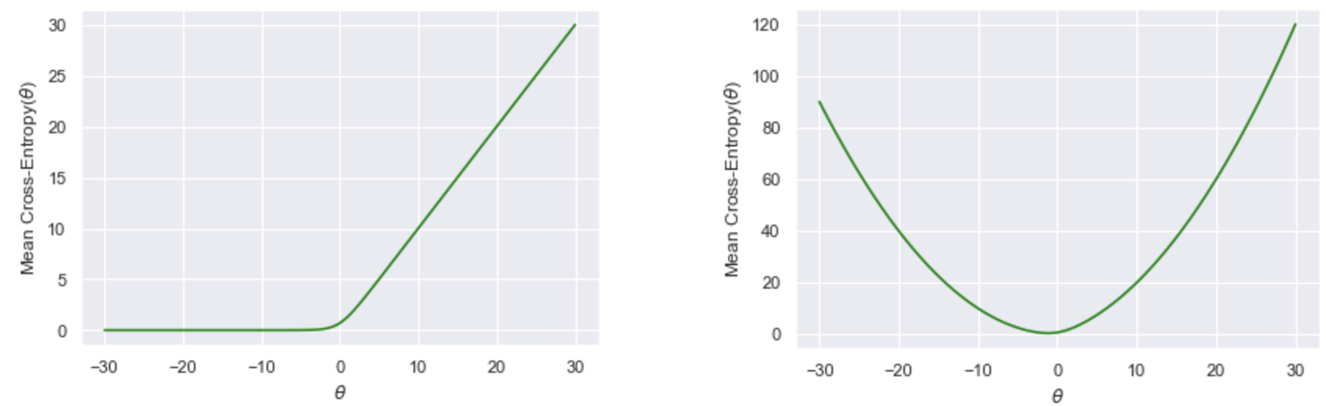
\includegraphics[scale=.4]{Bild47}
	    \end{figure}
	     Loss surfaces for linearly separable toy dataset from before.
	     \begin{itemize}
	         \item Left: no regularization.
	         \item Right: L2 regularization, with lambda = 0.1.
	     \end{itemize}
	 \end{frame}
	 
	 
	 \begin{frame}{Regularized logistic regression in scikit-learn}
	    \begin{itemize}
	        \item scikit-learn’s LogisticRegression package applies regularization by default.
	        \begin{itemize}
	            \item L2 by default, but you can change the penalty parameter.
	        \end{itemize}
	        \item But, its regularization hyperparameter C is the inverse of the lambda that we’ve discussed.
	        \begin{itemize}
	            \item C = 1 / lambda.
	        \end{itemize}
	        \item By default, C = 1.
	    \end{itemize}
	    
	   \\
	   \bigskip
	   LogisticRegression(C = 300)\\
	   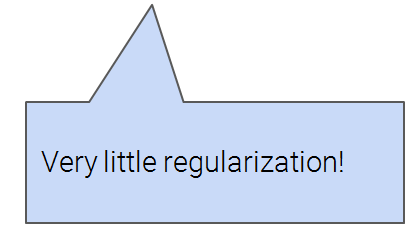
\includegraphics[scale=.5]{Bild48}

	 \end{frame}
\end{document}